\ifdefined\MThreeSmall
\documentclass[acmsmall,screen]{acmart}
\else
\documentclass[manuscript,screen,review]{acmart}
\fi
\usepackage{booktabs,tabularx,enumitem,amsmath}
\usepackage{seqsplit}
\usepackage{placeins}
\emergencystretch=1em
\usepackage{tikz}
\usetikzlibrary{arrows.meta,positioning}
\setcopyright{none}
\settopmatter{printacmref=false}
\acmJournal{TOMPECS}
\acmDOI{}
\acmYear{2026}
\title{Scheduler Rankings and Performance Trade-offs in a Common-Model LLM-Serving Evaluation}
\author{Soroush Vahidi}
\email{sv96@njit.edu}
\affiliation{\institution{New Jersey Institute of Technology}\city{Newark}\state{New Jersey}\country{USA}}
\newcommand{\cm}{CM-0.1}
\newcommand{\anwg}{\ensuremath{\mathrm{ANWG}}}
\newcommand{\authorreview}[1]{\par\noindent\textbf{AUTHOR REVIEW REQUIRED:} #1\par}
\begin{document}
\begin{abstract}
A scheduler comparison is difficult to interpret when its implementations
use different service, resource, or information rules. We evaluate four
project-maintained LLM-serving scheduler adaptations under a shared,
synthetic execution contract. The study covers 120 trace-derived windows
from three sources, six inherited arrival/deadline settings, and two KV
reservation capacities: 5,760 validated cells, all completing every request.
Against chunked-FCFS, the SLO-gated adaptation reduces the six source/capacity
aggregate mean latencies by 11.3--34.0\%, while reducing token throughput by
1.65--4.01\%. On BurstGPT, its mean window-level p95 latency increases by
3.72\% and 18.97\% at the two capacities. Its urgency gate does not bind;
these results concern the adaptation's admission ordering and chunking,
not the complete original SLAI algorithm. Chunked-FCFS and decode-first
produce identical records in all 1,440 matched conditions. No source-mean
comparison exhibits a strict 10\% practical reversal, although window-level
and metric-dependent reversals occur. Exact ties and redundant rankings
further limit what a leaderboard conveys. A separate 134,000-study
known-truth calibration diagnostic identifies failures of historical
inferential procedures under specified synthetic scenarios. The contribution
is a finite-corpus performance evaluation that distinguishes measured
trade-offs, model-implied invariances, and inferential limits; it is neither
a new scheduler nor a validated native-GPU performance predictor.
\end{abstract}
\ccsdesc[500]{Computing methodologies~Simulation evaluation}
\ccsdesc[300]{Computer systems organization~Cloud computing}
\keywords{LLM serving, performance evaluation, scheduling, trace-driven simulation, ranking stability}
\maketitle
\section{Introduction}
A serving scheduler can reduce average response time while making long
requests slower or lowering aggregate throughput. Which scheduler appears
best therefore depends on both the workload and the objective. There is a
more basic difficulty in simulation-based comparisons: a policy label can
select not only an ordering rule, but also a different prefill model,
memory constraint, or information interface. An observed rank difference
then combines scheduling decisions with differences in what the evaluator
allows those decisions to accomplish.

This problem arises in the historical LLM-Serving Scheduler Portability
(LSSP) corpus that motivates our study. Its implementations shared request
inputs, but did not uniformly enforce prefill work and KV capacity. Some
comparisons therefore concerned policy--model combinations rather than
scheduling alternatives within a common execution model. Repeating those
runs or reproducing their ranking arithmetic cannot resolve that ambiguity.
A useful comparison must first identify the execution contract: which
requests are visible, which actions are legal, how work advances, and when
resources are acquired and released.

We evaluate four adaptations under such a contract, \cm. It is a CPU
discrete-event model with common batch timing, token accounting,
information restrictions, and conservative full-context KV reservations.
The adaptations retain selected ideas from FCFS serving, chunked prefill,
decode-first scheduling, and SLAI-inspired prompt ordering
\citep{kwon2023vllm,agrawal2024sarathi,slai2025}. They have new implementation
identities and a shared action space. The purpose is to measure their
behavior under a controlled abstraction, not to reproduce the performance
of their published systems.

Workload-sensitive serving evaluations already establish that benchmark
choice matters \citep{papaioannou2024workload}; predictive serving simulators
address the cost of exploring configurations \citep{vidur2024,llmservingsim2024}.
Our contribution is a different empirical object: a complete comparison
of restricted adaptations across a fixed corpus, with absolute performance,
matched differences, ties, and practical reversals reported together.
This permits a reader to distinguish a useful performance difference from
a rank change caused by aggregation, duplicate metrics, or an inactive
scheduling distinction.

The completed comparison changes the emphasis of the historical narrative.
Across six source--capacity aggregates, SLO-gated improves mean latency but
reduces throughput; BurstGPT also has worse mean window-p95 latency.
Chunked-FCFS and decode-first are exactly equivalent in every matched
condition. Source-mean comparisons have no strict 10\% practical reversals,
whereas individual windows and different metrics do. These findings make
an unconditional ``best scheduler'' an inadequate summary, without implying
that rankings are unstable at every aggregation level.

We ask three questions:
\begin{description}[leftmargin=0pt,labelindent=0pt]
\item[RQ1: Performance and operating conditions.] How do the absolute
performances of four scheduler adaptations vary across workload windows,
inherited arrival/deadline settings, and KV reservation capacities?
\item[RQ2: Ranking stability and metric choice.] How do workload variation,
aggregation, metric selection, ties, and practical performance differences
affect scheduler rankings?
\item[RQ3: Interpretation and inference.] What do the historical comparison
audit and known-truth statistical calibration establish about the reliability
and limitations of scheduler comparisons?
\end{description}

The paper makes four specific contributions. First, it specifies an
executable comparison contract and identifies the departures of each
adaptation from its published lineage. Second, it reports the complete
5,760-cell evaluation, including absolute latency, throughput, goodput,
and complete request accounting. Third, it quantifies how window variation,
aggregation, ties, and metric choice change the interpretation of rankings,
including the null source-mean reversal result. Fourth, it separates
execution conformance from statistical calibration through a concise
historical audit and a completed synthetic diagnostic. These contributions
support finite-corpus conclusions under \cm; they make no new algorithmic,
statistical-test, or native-performance claim.

\FloatBarrier
\section{Related Work and Evaluation Scope}
\paragraph{Serving mechanisms.}
Orca introduced iteration-level scheduling to change batches as requests
progress \citep{yu2022orca}. vLLM's PagedAttention addresses KV-memory
fragmentation and sharing \citep{kwon2023vllm}. Sarathi-Serve uses chunked
prefill to manage throughput--latency trade-offs \citep{agrawal2024sarathi}.
Bari et al. distinguish the throughput-optimal RAD construction from the
practical SLAI scheduler, which uses measured decode urgency and known
prompt lengths \citep{slai2025}. These are system and algorithm contributions
with their own execution assumptions. Our whole-FCFS, chunked-FCFS,
decode-first, and SLO-gated adaptations isolate a smaller set of admissible
rules. In particular, full-context reservations do not reproduce
PagedAttention, and an inactive urgency gate supplies no evidence for
SLAI's complete design or RAD's theorem. Disaggregated serving and dynamic
migration, exemplified by DistServe and Llumnix
\citep{zhong2024distserve,sun2024llumnix}, are outside the single-device,
nonpreemptive contract evaluated here.

\paragraph{Workload-sensitive evaluation.}
Papaioannou and Doudali explicitly examine how dataset and inference-scenario
choice affect comparisons among LLM inference systems
\citep{papaioannou2024workload}. Their work is a close precedent for the
importance of workload choice, rather than a gap this paper first identifies.
Etalon identifies limitations of conventional latency and throughput
metrics for streaming user experience and introduces a fluidity index
\citep{agrawal2024etalon}. Our metric comparisons use the frozen aggregate
endpoints; they neither introduce a new user-experience metric nor measure
streaming fluidity.
BurstGPT contributes production-derived workload characterization
\citep{burstgpt2025}, and ServeGen studies production workloads and their
generation \citep{servegen2026}. Workload resampling has a longer history
in parallel-job scheduler evaluation \citep{zakay2014resampling}.
Our analysis instead holds a selected trace corpus fixed, matches each
adaptation on the same window and condition, and distinguishes source
means from cross-window comparisons. We do not infer that the selected
windows are independent draws from provider populations.

\paragraph{Throughput optimality and finite-window completion.}
Dai, Deng, Li, and Peng's May 18, 2026 revision studies batching and
work-conserving scheduling through queueing stability
\citep{dai2026throughput}. Their token-budget model has batch time depending
on token load; their maximal-batch-size extension shows that request-count
constraints materially change the stability analysis. This makes the
binding constraint a substantive modeling choice, rather than an incidental
configuration detail. In \cm, full-context reservations limit residency to
four or eight requests, chunked work cannot exhaust the token budget, and
every batch costs the same time. Moreover, our throughput is output from a
finite, fully drained input divided by its completion duration. It is not
their long-run stability criterion. Their work motivates examining batching
and concurrency together, but its theorems do not certify these adaptations;
our finite-window throughput losses neither refute their stability results
nor establish a new scheduling principle.

\paragraph{Related manuscripts and incremental question.}
Related active manuscripts by the author already study inactive mechanisms
and metric sensitivity. The action-opportunity/headroom manuscript asks when
an executable alternative exists and measures reference-conditional,
one-step causal value. The module-counterfactual manuscript studies typed
transplants, downstream erasure and transplant fidelity. The closed-API
resource-accounting manuscript separates nominal budgets, realized resources
and answer selection on different tasks and data. M3 does not contribute
those methods or reuse their quantitative results as validation. Its
incremental object is a complete common-contract adaptation comparison:
exact trajectory consequences for the chunked/decode pair, measured remaining
trade-offs, and the contrast between source-mean stability and window/metric
rankings, with a separate historical-inference diagnostic. The shared ideas
of explicit accounting and conditional mechanisms are acknowledged, not
claimed as unique to this paper. Appendix~\ref{app:evidence} and the related-
manuscript disclosure identify inspected local versions; actual submitted
versions and public citation identities require author confirmation.
M3 also reuses windows, reconstruction and the archived 36/990 rule result
from the earlier portability line, whose rejected/withdrawn submissions are
not active concurrent work.

\paragraph{Serving simulators and model credibility.}
Vidur combines profiling and predictive models to explore LLM inference
configurations \citep{vidur2024}; LLMServingSim develops HW/SW co-simulation
for serving workloads \citep{llmservingsim2024}. LLMServingSim 2.0 further
models interactions among runtime scheduling, heterogeneous hardware, and
disaggregated resources \citep{llmservingsim2026}. Those frameworks target
hardware-aware performance estimation and evaluate prediction accuracy.
\cm\ uses fixed-duration batches and an explicit work ledger to make
adaptations comparable and execution independently checkable. It cannot
replace their predictive objectives or borrow their validation evidence.
Following the distinction between verification and validation in simulation
methodology \citep{sargent2013}, reconstructing an execution journal tests
whether the program implements the declared model. Establishing adequacy
for a physical serving system would require separate evidence.

\paragraph{Statistical procedures.}
The calibration diagnostic uses existing procedures: Benjamini--Hochberg
(BH), Benjamini--Yekutieli (BY), Holm, and bounded concentration inequalities
\citep{benjamini1995,benjamini2001dependency,holm1979,hoeffding1963}.
Their assumptions do not follow from successful code execution. In
particular, a multiplicity adjustment cannot establish validity of its
input p-values or repair a mismatch between the tested null and a practical
performance claim. STAT01 investigates those issues in specified synthetic
scenarios; it does not propose a replacement test.

\FloatBarrier
\section{A Common Execution Contract}\label{sec:contract}
\subsection{Why the comparison object matters}
The historical corpus contains 9,360 configurations and two deterministic
verification passes per configuration. Its primary panel contains eleven
policies, with two additional style approximations. The historical engine
permits policy-dependent service modes: instantaneous prefill for some
policies, explicit prefill work for others, and differing enforcement of KV
limits. A policy's requested work can also differ from the engine's realized
progress. Consequently, those outcomes cannot be interpreted as a controlled
comparison of scheduling order. Table~\ref{tab:objects} distinguishes the
three evidence objects used in this paper.

\begin{table}[t]
\caption{Evidence objects and the conclusions they support. Historical
identifiers containing ``faithful'' are immutable names, not validation certificates.}
\label{tab:objects}\small
\begin{tabularx}{\linewidth}{@{}lXX@{}}\toprule
Object & Comparison or check & Interpretation \\\midrule
Historical LSSP & Policy-dependent service/resource modes; archived ranking arithmetic & Motivation and historical-rule counts \\
C01-FULL & Four adaptations; common \cm\ execution and information & Descriptive finite-corpus performance \\
STAT01 & Synthetic independent studies with known population truth & Scenario-specific inference calibration \\\bottomrule
\end{tabularx}
\end{table}

\subsection{Service, resources, and information}
\cm\ represents one abstract device. Each batch lasts 1\,ms and has a
32,768-token work budget. Each executed prompt token consumes one unit;
each selected decode request consumes one unit and emits one token.
All policies share these rules. A prefill batch emits no output, including
its final chunk: decoding can begin only in a later batch. Batch duration
is independent of its composition. Thus seconds and tokens per second
below are model quantities, not estimates for a particular GPU or LLM.

Each resident request reserves the complete 32,768-token context bound.
All frozen request lengths fit; the maximum prompt-plus-output length is
30,053. Capacities of 131,072 and 262,144 tokens therefore permit
\emph{four and eight resident requests}, respectively, even though the
configured sequence limit is 64. Actual used KV follows executed prompt
and output prefixes, rounded to 16-token blocks, and must remain within
the reservation. Completion releases the reservation. Waiting requests own
none. This conservative rule avoids output-length prediction and allocation
deadlock; it does not model incremental native paging or cache eviction.

There is no preemption, dropping, migration, prefix sharing, or recomputation.
Requests arriving during a batch become eligible at its end. Idle time
advances to the next arrival. The administrative horizon is the final
arrival plus 50\,s; a batch cannot finish beyond it. Unfinished requests
remain explicitly unfinished rather than contributing observed completion
latencies.

Policies see only arrived request identifiers, stable order, arrival time,
prompt length, acknowledged progress, residency, last-output/prefill-completion
anchor, and current time. Actual remaining output length, future arrivals,
source identity, and output-derived metric deadlines are hidden. The engine
either executes the exact proposed token spans or rejects the plan. The
shared contract therefore fixes both the resources and the online
information available to each adaptation.

\subsection{Adaptation identities and structural consequences}
Table~\ref{tab:policies} defines the four evaluated adaptations. Published
systems are lineage references; historical project implementations and
\cm\ adaptations are separate objects. The panel was targeted using the
historical comparison questions, not sampled to represent all schedulers.

\begin{table}[t]
\caption{Project-maintained adaptations. Artifact IDs append \texttt{\_c01}
to \texttt{whole\_fcfs}, \texttt{chunked\_fcfs}, \texttt{decode\_first}, and
\texttt{slo\_gated}. All use the shared contract above.}
\label{tab:policies}\small
\begin{tabularx}{\linewidth}{@{}p{.18\linewidth}p{.20\linewidth}X@{}}\toprule
Adaptation & Historical lineage & Executed ordering rule and principal restriction \\\midrule
Whole-FCFS & vLLM-inspired whole-prompt implementation & Admit whole prompts in arrival order when feasible; otherwise decode residents. Admitting prefills defers all decodes that batch. No native paged allocator. \\
Chunked-FCFS & vLLM-inspired chunked implementation & Resident work before waiting work in stable order; at most 512 prefill tokens per request per batch. \\
Decode-first & Sarathi-inspired implementation & Resident decodes, then resident prefills, then waiting prefills; 512-token cap. No original engine timing. \\
SLO-gated & SLAI-inspired implementation & Urgent decodes first; then resident prefills, waiting prefills by prompt length, and residual decodes. Fixed 0.495\,s gate; 512-token cap. No dynamic offset, heterogeneous classes, or full SLAI. \\\bottomrule
\end{tabularx}
\end{table}

Two consequences are essential to interpreting the results. At most eight
requests can execute, and each chunked request uses at most 512 tokens.
Their total work is therefore at most $8\times512=4,096$, below the shared
32,768-token budget. Every selected chunk and resident decode fits.
Chunked-FCFS and decode-first consequently make the same per-request
progress despite ordering their work differently. The complete saved
terminal records confirm this equivalence in all 1,440 matched conditions.

The same bound means that SLO-gated's residual decodes fit every batch.
After prefill completion, a resident's anchor advances with every output;
its elapsed time cannot reach the 0.495\,s urgency threshold in these
executions. The distinctive behavior is principally prompt-length admission
ordering with the frozen chunking rules. The results cannot be credited
to an active urgency gate. Whole-FCFS can still defer decoding for admitted
prefills; the work-bound equivalence does not apply to that rule.

\subsection{Conformance evidence}
The event referee reconstructs request states, token spans, timing,
completion, and resource use from the inputs and execution journal without
importing the engine or policy implementation. It checks that intended and
executed work agree and recomputes the metrics. Every campaign cell passed
this check; an independent analyzer also checked the complete ranking and
reversal reports. The final evidence review additionally checked all result
identities and terminal metrics and replayed 24 structurally selected new-cell
journals. These checks establish conformance to \cm, not GPU fidelity.
Figure~\ref{fig:contract} summarizes the evidence chain.

\begin{figure}[!htbp]
\centering
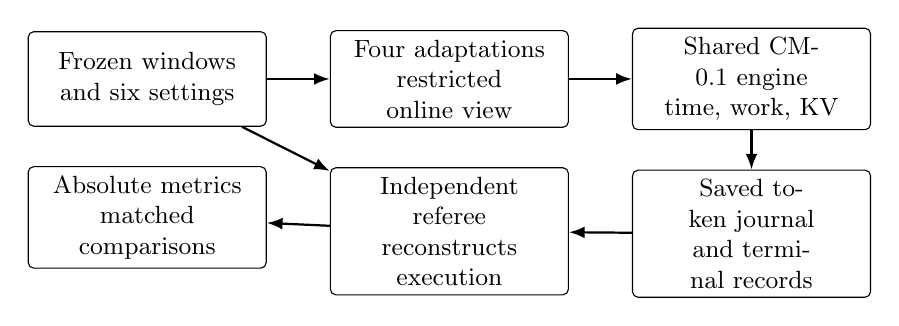
\begin{tikzpicture}[font=\small,node distance=5mm and 8mm,
 box/.style={draw,rounded corners=2pt,align=center,text width=.23\linewidth,minimum height=12mm},
 arr/.style={-{Latex[length=2mm]},thick}]
\node[box] (input) {Frozen windows\\and six settings};
\node[box,right=of input] (policy) {Four adaptations\\restricted online view};
\node[box,right=of policy] (engine) {Shared \cm\ engine\\time, work, KV};
\node[box,below=of input] (reports) {Absolute metrics\\matched comparisons};
\node[box,below=of policy] (referee) {Independent referee\\reconstructs execution};
\node[box,below=of engine] (journal) {Saved token journal\\and terminal records};
\draw[arr] (input)--(policy);\draw[arr] (policy)--(engine);
\draw[arr] (engine)--(journal);\draw[arr] (journal)--(referee);
\draw[arr] (referee)--(reports);\draw[arr] (input)--(referee);
\end{tikzpicture}
\caption{Comparison and verification under one model. The independent
analysis check recomputes aggregates, ranks, and reversals from the absolute
metrics. No stage in this chain establishes physical-system accuracy.}
\Description{Inputs pass through a restricted policy view and shared engine to a saved journal. An independent referee reconstructs execution before reporting metrics.}
\label{fig:contract}
\end{figure}

\FloatBarrier
\section{Corpus, Conditions, and Analysis}\label{sec:design}
\subsection{Trace and implementation provenance}
The corpus comprises 40 windows of 200 requests from each of Azure 2024,
Bailian/Qwen, and BurstGPT \citep{azure2024trace,bailianqwen2026,burstgpt2025}.
The Azure release identifies DynamoLLM as its accompanying publication
\citep{stojkovic2025dynamollm}; the pinned Bailian/Qwen release requests
attribution to the KVCache workload study \citep{wang2025kvcache}.
These are three separately released sources, not three independent provider
populations: BurstGPT and Azure have Azure infrastructure in their collection
provenance. Table~\ref{tab:provenance} identifies the consumed files and
transformations. The supplement records full file and window fingerprints.
The official Azure conversation release has the name
\texttt{AzureLLMInferenceTrace\_conv\_1week.csv}; its published SHA-256
matches the consumed file despite the local rename. Azure and BurstGPT
are licensed CC BY 4.0, and the pinned Bailian/Qwen data Apache 2.0.
Input acquisition instructions retain attribution, license texts, and
transformation notices. Public artifact distribution remains pending.

\begin{table}[t]
\caption{Consumed dataset provenance. Each row contributes 40 windows and
8,000 request records. Hashes are prefixes of SHA-256 values; full values are
in the bundled input manifest. The artifact provenance audit matches these hashes to upstream release
assets or a pinned LFS object and retains the corresponding license notices.}
\label{tab:provenance}\small
\begin{tabularx}{\linewidth}{@{}lXl@{}}\toprule
Source & File and representation & File hash prefix \\\midrule
Azure 2024 & \texttt{AzureLLMInferenceTrace\_conv\_2024.csv}; source arrival and token counts & \texttt{a0cc9b969a9b} \\
Bailian/Qwen & \texttt{qwen\_traceB\_blksz\_16.jsonl}; input/output lengths read directly; 16-token prefix-block hashes are separate fields & \texttt{68e3f98e2d60} \\
BurstGPT & \texttt{BurstGPT\_without\_fails\_2.csv}; retained valid source rows and token counts & \texttt{56193aa9b2bb} \\\bottomrule
\end{tabularx}
\end{table}

Each source's 40-window panel contains ten inherited pilot windows and 30
subsequent windows selected using fixed seeds and valid-row ranges. The
expanded manifest was frozen before its corresponding campaign outcomes;
earlier pilot outcomes already existed. Within the C01 manifest, row-overlap
checks find no overlapping selected ranges. Exact overlap with some related
projects' older BurstGPT selections remains unresolved. Nonoverlap within
this panel does not establish temporal independence or representativeness.
The frozen chronology labels allocate 20/10/10 windows per source to
EARLY/MIDDLE/LATE. Four consecutive ten-window blocks provide an additional
descriptive sensitivity; their elapsed time spans are unequal.

C01 reuses the historical input reconstruction, while its execution engine,
policy views, and adaptation implementations have separate identities.
C01-FULL retains C01 execution semantics at commit \texttt{9aed0206de66};
its full-campaign execution commit is \texttt{2d8342e699f3}.
The complete matrix has
$120\times6\times4\times2=5,760$ cells. Of these, 144 were reused from the
pilot only after matching input, code, configuration, and journal identities;
5,616 were newly executed in the completed full campaign. Reuse is not an
independent replication. No cell is omitted, and a deterministic cell is
not rerun to manufacture a sampling distribution.

\subsection{Inherited settings jointly transform arrivals and deadlines}
The six labels LOW, PRE\_KNEE, KNEE, POST\_KNEE, OVERLOAD, and HIGH\_PRESSURE
come from historical calibration, not from a saturation analysis of \cm.
For a window-specific compression factor $f$, rebased arrival gaps and
synthetic deadline slack are both divided by $f$. In idealized notation,
\begin{equation}
 a_i'=(a_i-a_1)/f,\qquad d_i'=a_i'+(d_i-a_i)/f.
\end{equation}
The implementation accumulates scaled nonnegative gaps in arrival order.
Prompt/output lengths and priorities are unchanged. Factors range from
22.525 to 180.873 for Azure, 17.956 to 186.580 for Bailian, and 102.884 to
725.020 for BurstGPT. Equal labels therefore do not mean equal absolute
arrival rates across windows or sources.

Deadlines are synthetic, derived in the inherited workload construction
using output-length information; priorities are uniform. These attributes
are not observed production service contracts. Deadlines are used only by
the metric layer and are hidden from the scheduling adaptations. The
setting axis is consequently \emph{joint arrival/deadline stress}. A change
in goodput across this axis cannot be attributed solely to arrival load.

\subsection{Endpoints and aggregation}
For arrival $a_i$, first output $u_i$, completion $c_i$, and output count
$o_i$, latency is $c_i-a_i$ and time to first token (TTFT) is $u_i-a_i$.
Time per output token (TPOT) is $(c_i-u_i)/(o_i-1)$ for $o_i>1$.
The saved means and p95s use their defined completed-request populations;
one-output requests do not have TPOT. The p95 uses the saved linear
interpolation convention. Completion fraction is completed requests divided
by all arrivals. Token throughput is completed output tokens divided by
elapsed time from first arrival to final completion, or to the horizon if
unfinished. Emitted-token throughput also counts any output of unfinished
requests. Request throughput uses the same time denominator.
These are finite-window completion rates, including the drain period;
they do not estimate a maximum sustainable arrival rate or system capacity.

Arrival-normalized weighted goodput is
\begin{equation}
 \anwg=\frac{\sum_i w_i\,\mathbf{1}\{i\text{ completes and }c_i\leq d_i'\}}
 {\sum_i w_i}.
\end{equation}
Here $w_i=1$, so \anwg\ is the fraction of arrivals meeting their synthetic
deadline. It is dimensionless, unlike requests or tokens per second.

The eleven frozen ranking endpoints are \anwg, completion fraction, three
throughput measures, and mean/p95 latency, TTFT, and TPOT. Larger is better
for goodput, completion, and throughput; smaller is better for the six
time endpoints. The complete endpoint set remains in the supplement,
including redundant and numerically uninformative endpoints.

The window is the principal analysis unit. At a fixed source, setting,
capacity, and policy, source means give each of the 40 windows equal weight.
For the compact source--capacity table, we first average the six settings
within each window and then average the 40 windows. A mean of window p95s
is always labeled as such; it is not a pooled-request p95. Matched differences
hold window, setting, and capacity fixed. We show all windows, not a selected
favorable subset.

\subsection{Ranking and practical-reversal definitions}\label{sec:reversal-rule}
Exact equality is primary: all maximizers or minimizers enter the top set,
and tied policies receive average ranks. The frozen sensitivity admits
values within $10^{-12}\max(1,|v_{\rm best}|)$ of the best; it does not
replace exact rankings or the practical-margin rule.

For policies $A,B$ and condition $c$, let
$\Delta_c=q_m(v_{A,c}-v_{B,c})$, where $q_m=1$ for a larger-is-better
endpoint and $q_m=-1$ otherwise. The relative margin is
\begin{equation}
 r_c=\frac{|v_{A,c}-v_{B,c}|}{|v_{\mathrm{loser},c}|}.
\end{equation}
A practical reversal between $c$ and $c'$ requires
$\Delta_c\Delta_{c'}<0$ and both $r_c>0.10$ and $r_{c'}>0.10$.
The strict boundary is evaluated exactly on the represented binary values.
Zero losing values and missing values are unestimable. Nonzero ties remain
eligible with margin zero. All denominators retain these distinctions.

Separate summaries compare within-source window pairs, Cartesian
cross-source window pairs, settings within a window, capacities at a fixed window and setting,
metrics at a fixed window, setting, and capacity, and source means
at a fixed setting/capacity/metric. Cross-source windows are not paired by
ordinal. For metric comparisons, each endpoint is oriented separately.
These overlapping comparisons describe the finite corpus. We attach no
population confidence intervals, p-values, or significance stars to C01.

\FloatBarrier
\section{Absolute Performance and Operating Conditions}\label{sec:performance}
\subsection{Completion and performance magnitudes}
All 5,760 cells complete all 200 requests. There is no administrative-horizon
censoring and no missing cell-level ranking endpoint. The 1,152,000 request
executions are repeated conditions on the 24,000 underlying records, not
independent observations. Individual TPOT excludes one-output-token
requests, leaving 103--200 observations per cell. Cell mean latency ranges
from 0.008314 to 3.893923 simulated seconds, p95 latency from 0.008560 to
7.300052 seconds, and output-token throughput from 332.489 to 7,766.685
tokens per simulated second. These magnitudes describe the fixed-cost model.

Figure~\ref{fig:absolute} shows every source/setting/capacity combination,
with equal-window means. Appendix Table~\ref{tab:absolute} gives compact
source/capacity aggregates. The SLO-gated adaptation reduces aggregate
mean latency relative to chunked-FCFS in all six source/capacity groups,
by 11.3--34.0\%. Yet token throughput falls by 1.65--4.01\% in those same
groups. On BurstGPT, mean window-p95 latency increases by 3.72\% with
four residents and 18.97\% with eight, despite better mean latency and
ANWG. On Bailian with four residents, ANWG decreases by 3.12\% despite
24.05\% lower mean latency. Lower average response time therefore does
not imply better tails, completion-by-deadline utility or throughput.

\begin{figure}[!htbp]
\centering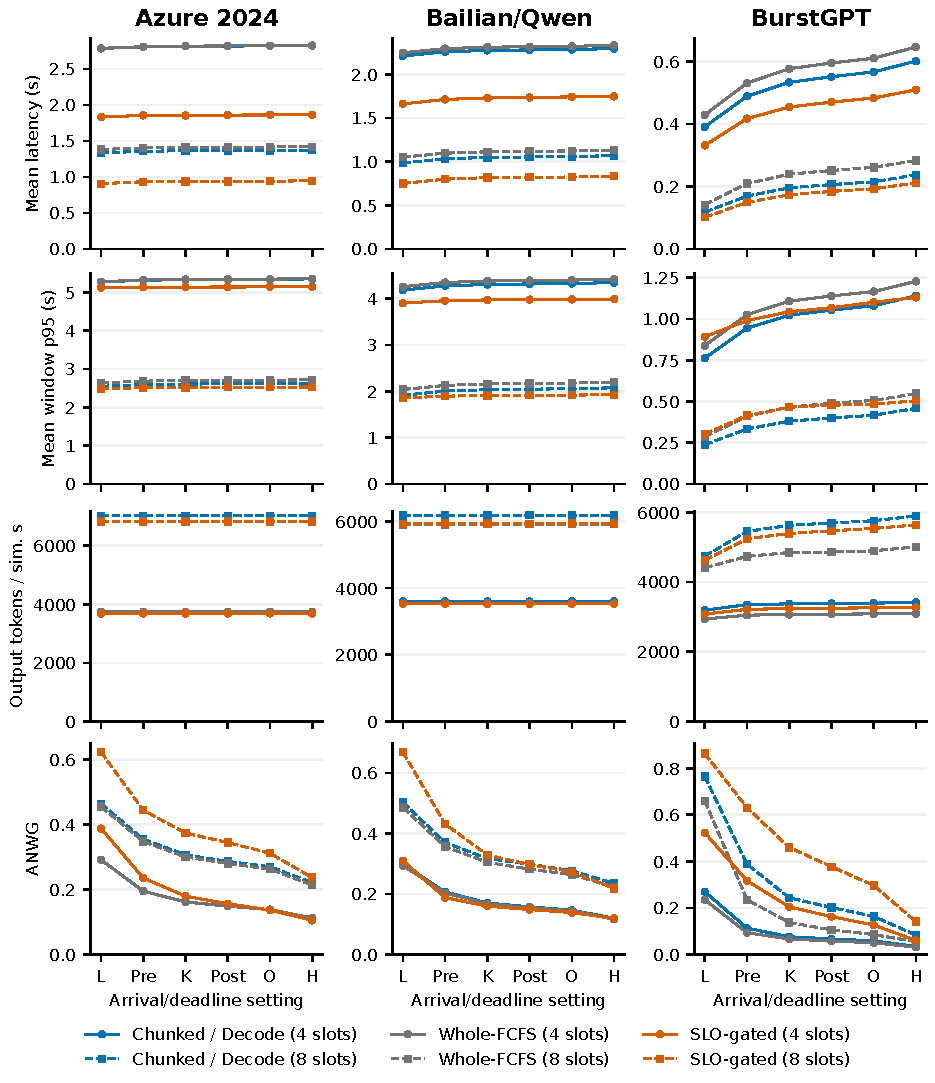
\includegraphics[width=\linewidth]{figures/absolute.pdf}
\caption{Absolute performance: 40 equally weighted windows per point.
L/Pre/K/Post/O/H denote the six inherited settings, not measured CM-0.1
saturation regimes. Solid/dashed lines allow four/eight reserved residents.
Chunked-FCFS and decode-first coincide exactly. Seconds and throughput
refer to simulated time; p95 panels average window-level p95s. No sampling
confidence intervals are implied.}\label{fig:absolute}
\Description{Twelve panels show mean latency, mean window p95 latency,
token throughput and ANWG by inherited setting for Azure, Bailian and
BurstGPT. SLO-gated has lower aggregate mean latency but lower throughput;
its BurstGPT tail latency is worse at both capacities.}
\end{figure}

\subsection{Matched-window trade-offs}
Figure~\ref{fig:matched} retains all 40 windows per source and both
capacities. Each point averages six \emph{matched differences} within a
window; it does not pool requests or substitute a difference between
unmatched supports. The combination of lower mean latency and worse tail
latency is visible on BurstGPT, while the size of the mean improvement
varies appreciably by window and capacity. Throughput losses accompany
many mean-latency improvements. Complete per-condition differences remain
in the frozen analysis, and the plotted window summaries are supplied as
CSV data.

SLO-gated is the unique mean-latency winner in 1,146 of 1,440 conditions,
but the unique p95-latency winner in only 834 and the unique token-throughput
winner in 482. Its unique ANWG wins number 1,004. The mean-latency count
splits into 480/480 Azure, 468/480 Bailian and 198/480 BurstGPT conditions.
These counts describe exact optima, not their practical margins. They
complement the absolute differences rather than override the unfavorable
throughput and tail outcomes.

\begin{figure}[!htbp]
\centering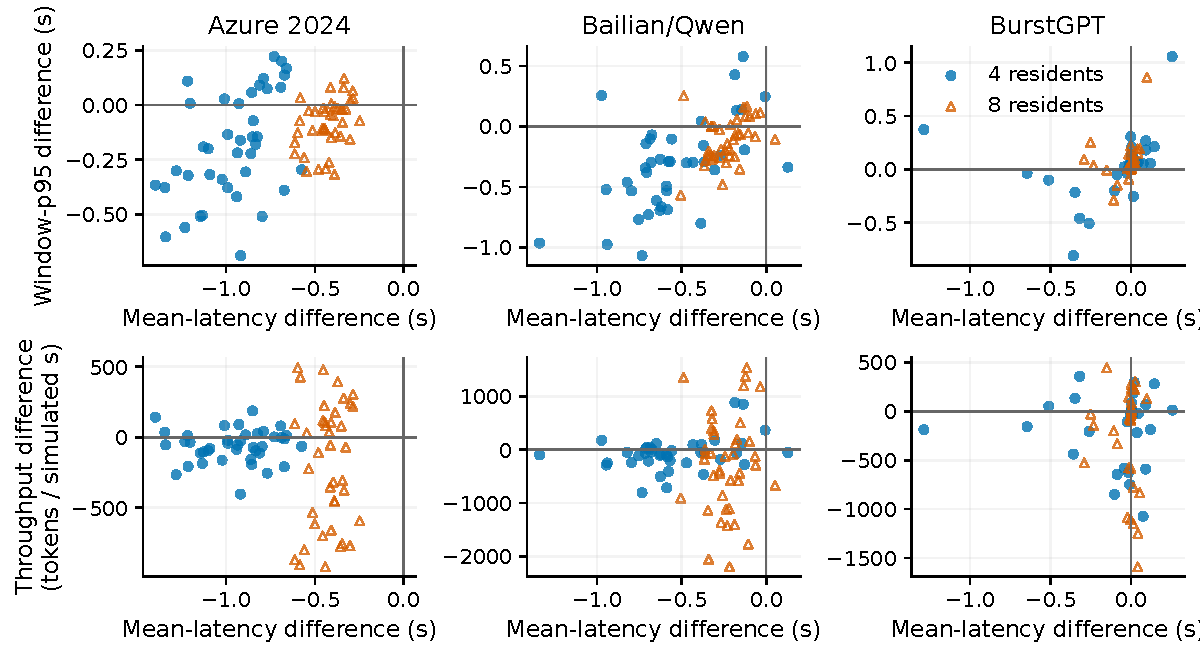
\includegraphics[width=\linewidth]{figures/matched.pdf}
\caption{SLO-gated minus chunked-FCFS for every window, averaged over its
six matched settings. Each panel has 40 windows at each of two capacities.
Leftward means lower mean latency; upward means worse window-p95 latency
(top) or higher throughput (bottom). These are descriptive points with no
independent-sampling interpretation.}\label{fig:matched}
\Description{Six scatter panels compare matched mean-latency differences
against p95 and throughput differences by source. Both capacity groups
and negative outcomes are retained.}
\end{figure}

\subsection{Reservation and setting sensitivity}
Doubling KV reservation capacity permits eight rather than four residents.
At the source/capacity aggregate level, this improves throughput and lowers
mean and mean-window-p95 latency for every adaptation. Actual used KV peaks
at 47,872 tokens in the smaller-capacity runs and 62,880 in the larger ones,
both below even the smaller nominal capacity. The observed constraint is
full-context reservation-induced concurrency, not exhaustion of used KV
at the nominal token limit. Paging, eviction and native memory-pressure
benefits cannot be inferred from this comparison.

Inherited settings can change goodput substantially while leaving aggregate
throughput almost unchanged. For Azure chunked-FCFS with four residents,
LOW to HIGH\_PRESSURE changes mean latency from 2.7858 to 2.8269 seconds
and token throughput from 3,745.9 to 3,746.3, while ANWG falls from
0.291375 to 0.112625. Equation~\ref{eq:scaling} explains why interpreting
this as an arrival-rate effect alone would be incorrect: the deadline
criterion becomes tighter at the same time.

\paragraph{Answer to RQ1.}
Under this reservation-limited contract, the complete corpus exhibits a
mean-latency/throughput trade-off with source-specific tail and goodput
costs. Capacity changes the permitted concurrency; inherited settings
jointly change arrivals and deadline slack. Completion is universal here,
so the reported trade-offs do not result from selectively omitting
unfinished requests. Their magnitudes are informative even where ranks
remain unchanged.

\FloatBarrier

\FloatBarrier
\section{Ranking Stability, Ties and Aggregation}\label{sec:rankings}
\subsection{Practical reversals depend on the comparison level}
Table~\ref{tab:reversals} retains every predeclared comparison axis and its
eligible denominator. There are \textbf{zero source-mean strict-10\%
practical reversals}. Nevertheless, source rankings need not coincide:
of 396 source-pair/setting/capacity/metric comparisons, 307 have identical
exact top sets, 323 have intersecting top sets and 247 have identical
full average-rank vectors. Differences below the practical threshold and
changes in ties coexist with the null practical-reversal result.

\begin{table}[t]\centering\small
\caption{Strict practical reversals across the complete panel. A reversal
exceeds 10\% relative to the losing value on both sides and changes sign.
Eligible counts retain nonzero ties; zero losing values are unestimable.
All comparisons are dependent descriptive enumerations.}\label{tab:reversals}
\begin{tabular}{lrrrr}\toprule
Axis & Reversals & Eligible & Unestimable & Total \\ \midrule
Within-source windows & 34,394 & 1,847,700 & 5,580 & 1,853,280 \\
Cross-source windows & 109,913 & 3,788,640 & 12,960 & 3,801,600 \\
Inherited settings & 920 & 236,853 & 747 & 237,600 \\
KV capacities & 350 & 47,418 & 102 & 47,520 \\
Metric choice & 11,795 & 473,580 & 1,620 & 475,200 \\
Source means & 0 & 2,376 & 0 & 2,376 \\
\bottomrule\end{tabular}

\end{table}

Window heterogeneity is not erased by stable source means. For ANWG alone,
within-source window comparisons produce 8,472 reversals among 162,900
eligible comparisons; cross-source windows produce 35,352/332,640.
The latter is a Cartesian comparison of windows, not pairing by ordinal.
ANWG setting and capacity comparisons yield 603/20,853 and 198/4,218,
respectively. A corpus-average recommendation therefore does not describe
every window or every utility. These are new adaptation/model estimands;
they do not demonstrate persistence of the 36 historical-rule records.

The raw pair counts must be interpreted with their constructions. Within
source, there are $\binom{40}{2}=780$ window pairs per stratum; between
sources there are $40^2=1600$. Settings generate 15 pairs, metrics 55,
and every comparison retains six policy pairs. Including the equivalent
chunked/decode-first pair preserves the frozen design, but its comparisons
cannot be counted as additional independent behavioral evidence. Comparing
these rates across axes is not a variance decomposition or a measure of
causal importance.

\subsection{Exact ties and metric redundancy}
The exact top set is tied in 425/1,440 ANWG conditions, 289/1,440
mean-latency conditions, 586/1,440 p95-latency conditions and 906/1,440
token-throughput conditions. Completion is tied everywhere. With every
request complete, emitted- and completed-token throughput coincide;
request throughput differs by a workload-specific constant within each
matched condition, so the three throughput rankings coincide as well.
They are distinct recorded quantities, not three independent confirmations.

Tiny timestamp differences create another reporting issue. The chunked
rules generate each resident output at essentially 1-ms intervals. The
largest cell mean-TPOT difference between chunked-FCFS and SLO-gated is
$1.80\times10^{-16}$ seconds. The predeclared near-tie sensitivity changes
the mean-TPOT maximizing set in 1,129/1,440 conditions and the p95-TPOT
set in 104/1,440. Exact records are preserved; such distinctions have no
practical performance interpretation. Appendix Table~\ref{tab:ties}
reports all eleven endpoints.

Across 79,200 metric-pair ranking comparisons, exact top sets agree in
27,915 and intersect in 57,602. The difference between these counts shows
why choosing one deterministic winner can obscure tied optima. Because
these totals include redundant endpoints and numerical TPOT distinctions,
the meaningful evidence is the absolute mean/tail/throughput trade-off,
not the metric-pair disagreement count alone.

\subsection{Chronological sensitivity}
The four ten-window blocks preserve variation hidden by source-wide
aggregation (Appendix Figure~\ref{fig:chronology}). SLO-gated minus
chunked-FCFS ANWG block means range from $-0.0120$ to $0.2030$ for Azure,
$-0.0300$ to $0.2330$ for Bailian and $0.0150$ to $0.3275$ for BurstGPT.
Negative differences occur in 8/48, 24/48 and 0/48 block/setting/capacity
combinations, respectively. The frozen early/middle/late partitions give
negative differences in 6/36, 20/36 and 0/36 corresponding combinations.
These partitions have unequal durations and related windows; the counts
describe the corpus ordering, not confidence about future workload shifts.

\paragraph{Answer to RQ2.}
Practical ordering is stable across source means at the frozen threshold,
but window and metric comparisons reveal changes that those means hide.
Exact ties, equivalent adaptations and redundant or numerically sensitive
metrics make a single leaderboard incomplete. Absolute differences and
set-valued optima explain more than a count of nominal rank changes.

\FloatBarrier
\section{Supporting Historical Interpretation and Calibration}\label{sec:inference}
\subsection{What the historical comparison establishes}
The historical analysis reported 36 of 990 policy-pair/source-pair/setting
records meeting its practical-margin and nominal-interval rule. Numerical
reproduction confirms that archived-rule count. It does not establish
population reversals: the historical policy--model combinations differ,
selected trace windows have no known population sampling law, and the
inference procedure's calibration was unestablished. The C01 panel and
execution model change the comparison object, so its zero source-mean
practical reversals are not a like-for-like disappearance of those 36
records. Historical and common-model outcomes are kept in separate evidence
strata rather than combined into a leaderboard.

\subsection{A focused known-truth diagnostic}
STAT01 evaluates historical inference in synthetic studies whose population
means, covariance, and missingness are specified. Each study has three
sources, eleven policies, and normally 40 windows per source; one bounded
scenario uses 400. The 165 source-pair/policy-pair hypotheses are dependent
within a study. Independently generated studies, not their individual
hypotheses, are the Monte Carlo units. The completed design contains
134,000 studies across 18 scenarios, including independent and identically distributed (IID), block-dependent,
autoregressive, nonnormal, bounded, and missing-data cases.

The primary truth is a population reversal exceeding 10\% relative to the
losing mean in both sources. Sign reversals are a separate endpoint.
The historical procedure first screens noisy point estimates at 10\%, then
uses bootstrap intervals and zero-effect p-values on the selected contrasts.
Testing a zero-effect null after such screening is not automatically a
test of the practical-effect null. Benjamini--Hochberg (BH) or Benjamini--Yekutieli (BY) adjustment alone cannot supply the missing
calibration \citep{benjamini1995,benjamini2001dependency}.

Three implementation identities are retained. The eight frozen original
procedures include a port of the historical screened-BH procedure. A
post-diagnosis comparator reproduces the actual historical source's
floating-point evaluation order. Eight additional comparisons implement
explicit mathematical threshold semantics. Thus the expanded family has
17 methods, with nine additions identified as post-diagnosis. Arithmetic
correction is not a new test and does not change the inferential assumptions.
Appendix~\ref{app:stat} gives the definitions and the saved boundary case.

\begin{table}[t]
\centering\small\setlength{\tabcolsep}{3pt}
\caption{Compact calibration diagnostic for the actual historical-source
screened-BH comparator. Each row has 8,000 studies; ordinary fixed-contrast
interval coverage is available in all of them. Bounds are the expanded
17-method simultaneous Monte Carlo bounds, not confidence intervals for
C01 performance. These three null scenarios isolate IID, independent-block,
and autoregressive (AR) dependence; all 18 scenarios and methods remain in the supplement.}
\label{tab:calibration}\begin{tabular}{lrrrr}
\toprule
Scenario & FDR & MC bounds & Coverage & MC bounds \\
\midrule
IID equal null & 0.09025 & [0.06878, 0.11172] & 0.94187 & [0.92357, 0.96018] \\
Independent-block null & 0.91800 & [0.89726, 0.93874] & 0.64762 & [0.61465, 0.68060] \\
AR(0.7) null & 0.98037 & [0.96780, 0.99295] & 0.56487 & [0.53081, 0.59894] \\
\bottomrule
\end{tabular}

\end{table}

Table~\ref{tab:calibration} shows that the actual historical-source procedure
has practical false-discovery rate (FDR) 0.09025 in the IID equal-null scenario, with an expanded
Monte Carlo lower bound above 0.05. Independent-block and AR nulls show
much larger false-discovery rates and poor ordinary interval coverage.
These null examples already demonstrate a calibration concern without
requiring interpretation of power or near-boundary alternatives.

Appendix~\ref{app:stat} retains all classifications, stopping counts,
original-eight and expanded-17 uncertainty families, abstentions, precision
gaps, and low-power outcomes. These qualify the calibration findings.

\paragraph{Implication for the common-contract study.}
Reproducing historical arithmetic establishes what its rule reported;
execution conformance establishes that C01 follows its common model.
Neither establishes valid statistical inference. STAT01 demonstrates
calibration failures for historical procedures in explicit known-truth
scenarios, while retaining uncertainty and assumption-specific limits.
C01's finite-corpus descriptions do not depend on population significance tests.

\FloatBarrier
\section{Discussion and Threats to Validity}\label{sec:discussion}
\paragraph{What an evaluator should report.}
The useful comparison object is an adaptation together with its execution,
resource, and information contract. A common contract exposes both
nontrivial trade-offs and distinctions that cannot affect execution.
Here, the budget and reservation rules collapse chunked-FCFS and
decode-first to one behavior and leave the urgency gate inactive. Reporting
four implementation names without these consequences would overstate
mechanistic coverage. Absolute latency and throughput then reveal costs
that a goodput-only or mean-latency-only ranking would miss.
The comparison is informative partly because it identifies which nominal
choices have no executable consequence under the stated constraints.
Its remaining empirical question concerns admission order, chunked versus
whole prefill, and residency, rather than a broad contest among native
serving algorithms. Changing the budget, timing model, or resource contract
could restore distinctions; this study makes no measured claim about those
unevaluated configurations.

Aggregation must be specified with the same care. A source mean answers a
question about equal-window average performance; a cross-window reversal
asks whether two particular windows prefer different policies. Neither
supersedes the other. A reader selecting a scheduler for variable traffic
needs both the aggregate magnitude and its window-level variation. Exact
top sets retain ties, and a practical margin prevents negligible numerical
differences from becoming performance claims.

\paragraph{Model adequacy and external validity.}
\cm\ deliberately fixes batch duration, assigns equal work units to prompt
and decode tokens, reserves a full context before execution, and omits
preemption and migration. It does not model kernel costs, bandwidth,
communication, native allocation, model-dependent token timing, or changing
batch efficiency. Its latency and throughput values describe the abstraction.
Independent event conformance and deterministic replay cannot establish
physical prediction accuracy \citep{sargent2013}. Related native probes
and other projects' mechanism studies do not validate this four-adaptation
ranking matrix. No deployment recommendation follows directly from it.

\paragraph{Corpus and construct validity.}
The 120 selected windows are finite and temporally related. They represent
particular files, valid-row filtering, and sampling rules rather than
random samples of providers. The two Azure-linked sources should not be
treated as independent providers, and cross-project overlap of some older
BurstGPT selections is unresolved. Uniform priorities and synthetic,
output-derived deadlines restrict the interpretation of \anwg. The inherited
setting transformation changes deadlines together with arrivals. Full-context
reservation capacity measures a residency constraint, and the panel excludes
many mechanisms available to production engines. These restrictions bound
which workload and resource questions the study answers.

\paragraph{Verification and inferential validity.}
Independent checks reduce the risk that reported metrics disagree with the
model or saved records; they cannot remove assumptions shared by the model
and the scientific question. The final review checked every result identity
and metric summary, while fresh journal replay sampled 24 new cells in
addition to the exhaustive in-campaign referee. C01's descriptive scope
avoids unsupported sampling assumptions but does not imply population
robustness. STAT01 supplies known truth only for its specified generators.
Its post-diagnosis additions, finite study counts, conditional interval
availability, and conservative power must remain visible when interpreting
calibration screens.

\section{Conclusion}
Under a common execution contract, scheduler comparison is as much about
performance magnitudes and inactive distinctions as about the rank order.
For RQ1, SLO-gated reduces aggregate mean latency by 11.3--34.0\% but loses
throughput, with worse BurstGPT mean window-p95 latency; chunked-FCFS and
decode-first are identical throughout the evaluated matrix. For RQ2, no
source-mean comparison has a strict 10\% practical reversal, while window
and metric comparisons do, and many exact rankings are tied or redundant.
For RQ3, the historical audit and synthetic diagnostic distinguish
reproducible execution and arithmetic from calibrated inference. The
result is a bounded, traceable performance evaluation: its strongest
conclusions concern the measured trade-offs and invariances of these
adaptations under \cm.

\FloatBarrier
\section*{Artifact Availability and Author-Review Items}
The M3 review package contains source, figures, tables, saved analysis
summaries, SHA-256 fingerprints, generation scripts, and both ACM manuscript
and \texttt{acmsmall} PDFs. A separate local versioned candidate assembles
the pinned C01 and STAT01 code, complete saved campaign records, frozen
inputs, source-data copies, license notices, and portable verification
recipes. Supplementary CSVs retain all 5,760 C01 cells and all 7,200 final
STAT01 endpoint summaries across the original and expanded families.
Saved-data verification and display regeneration generate no new experiment.
The rc1 candidate is unchanged and contains the earlier manuscript snapshot.
A versioned local companion supplies this revised manuscript and example
support, with checksums and pairing instructions; it reuses rc1 raw evidence.
Neither candidate nor companion has been externally released.

\authorreview{Approve reviewer access and immutable release identifiers for
the local candidate. The provenance audit independently matches all three
consumed source hashes to official release assets or a pinned LFS object:
Azure and BurstGPT are CC BY 4.0, and Bailian/Qwen Apache 2.0. Approve the
accompanying attribution/change notices and the compilation/code/synthetic-data license scopes and retention plan;
verified source terms do not constitute authorization to publish this candidate.}
\authorreview{The author's correspondence review verifies that the JSC
portability submission was rejected September 28, 2026, its PEVA version
October 2, and the SIMPAT version October 21; LLM6030 withdrawal was confirmed
September 18. These are not active concurrent submissions. Approve attribution
of reused historical windows, reconstruction and results, and the distinction
from the active headroom paper (PEVA-D-26-00474), module-counterfactual paper
(SIGMETRICS 2027 \#5), and closed-API resource-accounting paper
(PEVA-D-26-00351, last confirmed under review August 19).
Approve the related-manuscript disclosure and stable version identities;
exact older BurstGPT overlap remains unresolved.}
\authorreview{Confirm the complete author list, contact/affiliation,
contribution roles, competing interests, funding and in-kind support.
Proposed statements with explicit confirmation fields are in the artifact
release documentation; no absence of funding or conflicts is presumed.}
\authorreview{Codex assisted manuscript preparation, saved-data displays,
code inspection, artifact packaging and validation reports. Confirm the
complete research-AI history, including earlier experimental code/analysis,
and finalize a methods disclosure and human-responsibility statement.
ACM's May 2026 policy distinguishes research-AI use from writing assistance.
Confirm current official ToMPECS initial-review format, anonymity, length
and supplement rules: its author-guidelines endpoint remains inaccessible.
The official ACM template maps TOMPECS to \texttt{acmsmall}, but no
journal-specific page limit or initial-review requirement is inferred.}

\FloatBarrier
\bibliographystyle{ACM-Reference-Format}
\bibliography{references}
\clearpage
\appendix
\section{Complete Performance and Ranking Context}\label{app:results}
\begin{table}[t]\centering\small
\caption{Equal-window source/capacity means, after averaging the six settings
within each window. R is the number of full-context residents (4/8 for
131,072/262,144 token capacity). Latency columns are seconds; p95 is the
mean of window p95s. Throughput is output tokens per simulated second.
Chunked and decode-first are combined only for display; all four identities
remain in the saved tables.}\label{tab:absolute}
\begin{tabular}{lllr r r r}\toprule
Source & R & Adaptation & ANWG & Mean & p95 & Throughput \\ \midrule
Azure 2024 & 4 & Whole-FCFS & 0.1746 & 2.8145 & 5.3275 & 3743.5 \\
Azure 2024 & 4 & Chunked / Decode & 0.1746 & 2.8132 & 5.3232 & 3746.2 \\
Azure 2024 & 4 & SLO-gated & 0.2001 & 1.8559 & 5.1342 & 3684.4 \\
Azure 2024 & 8 & Whole-FCFS & 0.3101 & 1.4092 & 2.6892 & 6816.5 \\
Azure 2024 & 8 & Chunked / Decode & 0.3174 & 1.3626 & 2.5986 & 7018.7 \\
Azure 2024 & 8 & SLO-gated & 0.3892 & 0.9357 & 2.5131 & 6825.8 \\
Bailian/Qwen & 4 & Whole-FCFS & 0.1799 & 2.3020 & 4.3705 & 3548.3 \\
Bailian/Qwen & 4 & Chunked / Decode & 0.1828 & 2.2655 & 4.2969 & 3603.2 \\
Bailian/Qwen & 4 & SLO-gated & 0.1771 & 1.7205 & 3.9681 & 3531.4 \\
Bailian/Qwen & 8 & Whole-FCFS & 0.3189 & 1.1063 & 2.1463 & 5914.1 \\
Bailian/Qwen & 8 & Chunked / Decode & 0.3330 & 1.0417 & 2.0227 & 6183.4 \\
Bailian/Qwen & 8 & SLO-gated & 0.3693 & 0.8087 & 1.9037 & 5935.7 \\
BurstGPT & 4 & Whole-FCFS & 0.0889 & 0.5654 & 1.0843 & 3054.9 \\
BurstGPT & 4 & Chunked / Decode & 0.1030 & 0.5225 & 1.0005 & 3354.9 \\
BurstGPT & 4 & SLO-gated & 0.2321 & 0.4448 & 1.0377 & 3223.4 \\
BurstGPT & 8 & Whole-FCFS & 0.2129 & 0.2314 & 0.4505 & 4796.5 \\
BurstGPT & 8 & Chunked / Decode & 0.3072 & 0.1907 & 0.3707 & 5532.1 \\
BurstGPT & 8 & SLO-gated & 0.4613 & 0.1692 & 0.4410 & 5322.3 \\
\bottomrule\end{tabular}

\end{table}

\begin{table}[t]\centering\small
\caption{All frozen ranking endpoints: counts out of 1,440 matched
conditions. ``Sensitivity changes'' compares the frozen near-tie top set
with the exact top set; it does not alter the practical-reversal rule.}
\label{tab:ties}
\begin{tabular}{lrrr}\toprule
Endpoint & Tied exact top & Sensitivity changes & Missing \\ \midrule
ANWG & 425 & 0 & 0 \\
Completion & 1,440 & 0 & 0 \\
Completed-token throughput & 906 & 0 & 0 \\
Emitted-token throughput & 906 & 0 & 0 \\
Request throughput & 906 & 0 & 0 \\
Mean latency & 289 & 6 & 0 \\
p95 latency & 586 & 0 & 0 \\
Mean TTFT & 286 & 2 & 0 \\
p95 TTFT & 488 & 0 & 0 \\
Mean TPOT & 979 & 1,129 & 0 \\
p95 TPOT & 1,348 & 104 & 0 \\
\bottomrule\end{tabular}

\end{table}

\begin{figure}[!htbp]\centering
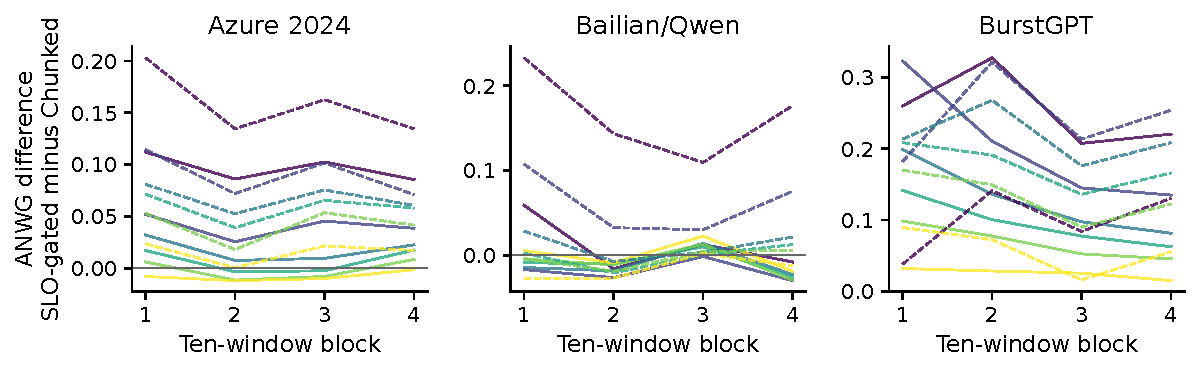
\includegraphics[width=\linewidth]{figures/chronology.pdf}
\caption{SLO-gated minus chunked-FCFS ANWG in four consecutive ten-window
blocks per source. Color advances from LOW (purple) to HIGH\_PRESSURE
(yellow); solid/dashed denotes four/eight residents. Each line fixes a
setting/capacity. Blocks are ordered corpus partitions, not equal-duration
or independent samples.}\label{fig:chronology}
\Description{Three panels plot all twelve setting/capacity series across
four blocks. Azure and Bailian include negative differences; BurstGPT
has positive differences throughout.}
\end{figure}

The supplement's \texttt{all-cell-metrics.csv} contains all 5,760 rows,
all accounting metrics and their condition, request, result and journal
hash references. \texttt{source-capacity-means.csv} retains all four
adaptations and all eleven ranking endpoints.
\texttt{matched-window-differences.csv} and
\texttt{chronological-differences.csv} contain the exact displayed
values. All six reversal axes and every exact/near-tie count are supplied
as CSV tables. Original per-setting source means, ranks and detailed
reversal groups remain in the hash-verified saved JSON reports.

\FloatBarrier
\section{Statistical Diagnostic Definitions and Full Scenario Accounting}\label{app:stat}
\subsection{Known truth and method identities}
Each synthetic study contains $Y_{sjw}$ for three sources, eleven policies
and normally 40 windows per source. The final bounded scenario has 400
windows. Sources and successive studies are independent by construction;
within-study windows and policies can be dependent. Positive population
means define the strict practical alternative for source pair $(s,t)$ and
policy pair $(a,b)$ as
\begin{align}
 &(\mu_{sa}>1.1\mu_{sb}\ \land\ \mu_{tb}>1.1\mu_{ta})\nonumber\\
 &\quad\lor(\mu_{sb}>1.1\mu_{sa}\ \land\ \mu_{ta}>1.1\mu_{tb}).
\end{align}
Equality at the boundary is null. Sign truth instead tests whether the
two mean differences have opposite signs. The 165 hypotheses are
$\binom{3}{2}\binom{11}{2}$ overlapping contrasts, not independent studies.

The default generator has Gaussian innovations, noise scale 0.15 and
cross-policy correlation 0.5. Window covariance is IID, independent
five-window blocks with correlation 0.7, or AR(1) with coefficient 0.7.
Equal means are 0.5; stable/near-tie means are $0.5+0.01j$ and
$0.5+0.0002j$. Reversal cases swap policies 0/1 between sources 0/1 at
$0.5\pm\delta/2$, leaving other means 0.5. Small, medium and large
reversals use $\delta=0.03,0.10,0.30$; dependence, variance and missingness
reversals use 0.15. The practical boundary swaps 0.55 and 0.5. Exact ties
use perfectly shared policy noise. Unequal scales are $(0.08,0.25,0.15)$;
the mixed case combines standardized Gaussian, $t_5$ and lognormal
innovations. MCAR masks observe each policy/window independently with
probability 0.8; the selective null hides below-mean source-0/policy-0
and source-1/policy-1 outcomes. Bounded cases use IID standardized uniform
innovations, scale 0.08 and $\delta=0.30$, analytically within $[0,1]$.
No latent missing values are imputed into an analysis.

\begin{table}[t]\centering\small
\caption{Eight original procedure IDs, abbreviated in Table~\ref{tab:scenarios}.
All have nominal $\alpha=q=0.05$. Historical methods use point screening
and zero-effect bootstrap components; the other reversal procedures test
practical contrasts and account for both orientations.}\label{tab:statmethods}
\begin{tabularx}{\linewidth}{lX}\toprule
Code & Frozen procedure and scope\\\midrule
HS & \texttt{historical\_screened\_BH}: practical point screen, 2,000
bootstrap draws, max of two source tail fractions, screened-family BH,
both percentile intervals exclude zero.\\
HF & \texttt{historical\_full\_BH}: same screened p-values; untested values
set to one in the full 165-hypothesis family.\\
HB & \texttt{historical\_plus1\_BY}: plus-one tail adjustment and full-family
BY; component and selection limitations remain.\\
T & \texttt{iid\_t\_Holm}: paired practical-contrast Student tests;
Gaussian IID complete/MCAR samples.\\
CT & \texttt{cluster\_t\_Holm}: tests on completely observed five-window
cluster means; Gaussian independent clusters; fewer than two clusters abstains.\\
O & \texttt{oracle\_normal\_Holm}: known covariance of matched means;
Gaussian complete/MCAR samples, including specified dependence.\\
G & \texttt{group\_bootstrap\_BY}: centered bootstrap over nonoverlapping
five-window groups, retaining masks; no asserted finite-sample guarantee.\\
B & \texttt{bounded\_Hoeffding\_Holm}: independent bounded samples only;
abstains elsewhere.\\\bottomrule
\end{tabularx}
\end{table}

For the nonhistorical procedures, a directional reversal requires both
source components, giving the maximum of their one-sided p-values. The
two possible orientations are combined by $\min(1,2\min(p_1,p_2))$ before
full-family adjustment. The bounded procedure uses Hoeffding's inequality
\citep{hoeffding1963} for $Z=Y_a-1.1Y_b\in[-1.1,1]$, with component
$p=\exp[-2n\max(\bar Z,0)^2/2.1^2]$. Valid component assumptions are
essential; Holm or BY does not supply them.

An additional \texttt{legacy\_source\_screened\_BH} preserves the actual
historical code. Eight \texttt{exact\_} counterparts correspond one to one
to Table~\ref{tab:statmethods}. All nine are post-diagnosis additions;
none replaces an original result or drives its stopping rule. For ordered
finite probabilities, exact BH rejects through the largest rank satisfying
$p_{(i)}\le i\alpha/m$, BY uses $i\alpha/(mH_m)$ with rational
$H_m=\sum_{j=1}^m1/j$, and Holm rejects successively while
$p_{(i)}\le\alpha/(m-i+1)$, with $\alpha=1/20$
\citep{benjamini1995,benjamini2001dependency,holm1979}.

Historical bootstrap probabilities are reconstructed as $2k/2000$ only
when the frozen floating expression reproduces the saved value exactly.
Plus-one values are $\min(1,(2k+2)/2001)$; grouped-bootstrap values use
$\min(1,2k/2001)$ with $k\ge1$. Analytic probabilities are exact dyadic
representations of the saved finite binary64 numbers, not infinitely
precise analytic tails. Nonfinite or off-grid inputs are rejected; there
is no boundary tolerance. Exact comparisons use independent rational
adjusted-p oracles, while legacy tests execute SHA-verified historical
source and preserve its stable-sort/missingness behavior.

\subsection{Uncertainty, stopping and endpoint denominators}
For each independent study, $R$ is the number of discoveries, $V$ the
number false under a specified truth, and FDP is $V/\max(R,1)$. FDR is its
expectation, FWER is $P(V>0)$, and power is the true-discovery fraction
when alternatives exist. Both sign and practical truth are retained.
Ordinary diagnostic coverage concerns the predeclared source-0,
policy-0-minus-policy-1 mean difference. Selected-interval coverage is
separate and conditional on emitting intervals; unavailable intervals
remain missing. For example, cluster-t emits ordinary intervals in only
1,676/8,000 MCAR studies and 202/8,000 selective-null studies. In the IID
equal null, historical selected coverage is 0.123834 over 958 emitting
studies, compared with 0.941875 ordinary diagnostic coverage over 8,000.
These are not interchangeable denominators or pooled independent intervals.

The finite analysis looks are 500, 1,000, 2,000, 4,000 and 8,000 studies
per scenario. For a bounded study endpoint with sample variance $s^2$ and
available count $N\ge2$, the two-sided empirical-Bernstein half-width is
\begin{equation}
 b=\sqrt{\frac{2s^2\log(4/\delta)}{N}}
   +\frac{7\log(4/\delta)}{3(N-1)}.
\end{equation}
Bounds clip $\bar X\pm b$ to $[0,1]$; counts below two receive the full
interval. This follows the bounded independent-observation inequality
and its two-sided union accounting \citep{maurer2009}. Original summaries
allocate $\delta=0.05/(18\cdot8\cdot16\cdot5)$; expanded summaries allocate
$0.05/(18\cdot17\cdot16\cdot5)$ to every included method. Endpoint
independence is not required for that finite union bound. Conditional
coverage uses the IID emitted-study population and its available count.
For post-diagnosis methods the statement is conditional on the fixed
amended family; it does not protect arbitrary data-dependent method search.

Only the original eight methods determine stopping: required half-widths
are at most 0.025 for practical FDR, FWER and null rejection fraction,
0.03 for ordinary coverage and 0.08 for power when defined. Precision is
not a calibration verdict. Table~\ref{tab:scenarios} includes every scenario
and the actual final stop. Seven of its nine empirical-compatibility entries
are exact-tie cases; the other two are conservative bounded procedures.
Across all 144 original method/scenario cells there are 45 concerns,
74 inconclusive results, nine compatible-with-tolerance results and
16 outside-domain abstentions.

\begin{table}[t]\centering\small
\caption{Complete original-family scenario accounting. P: precision
objective met; M: maximum count with precision gaps. C: FDR lower bound
$>0.05$ or ordinary-coverage upper bound $<0.95$; E: FDR upper bound
$\le0.06$ and coverage lower bound $\ge0.94$; I: inconclusive; A: outside-domain
abstention. E permits conservative overcoverage and is not exact nominal
calibration. Abbreviations follow Table~\ref{tab:statmethods}.}
\label{tab:scenarios}
\begin{tabular}{lrrcccccccc}\toprule
Scenario & Studies & Stop & HS & HF & HB & T & CT & O & G & B \\ \midrule
0: IID equal null & 8,000 & P & C & I & I & I & I & I & C & A \\
1: IID stable null & 8,000 & P & I & I & I & I & I & I & C & A \\
2: IID near ties & 8,000 & P & C & I & I & I & I & I & C & A \\
3: Exact policy ties & 2,000 & P & E & E & E & E & E & E & E & A \\
4: Practical boundary & 8,000 & M & C & I & I & I & I & I & C & A \\
5: Small sign reversal & 8,000 & M & C & I & I & I & I & I & C & A \\
6: Medium reversal & 8,000 & M & C & C & I & I & I & I & C & A \\
7: Large reversal & 8,000 & M & I & I & I & I & I & I & C & A \\
8: Block null & 8,000 & M & C & C & C & C & I & I & C & A \\
9: Block reversal & 8,000 & M & C & C & C & C & I & I & C & A \\
10: AR null & 8,000 & M & C & C & C & C & C & I & C & A \\
11: AR reversal & 8,000 & M & C & C & C & C & C & I & C & A \\
12: Unequal variances & 8,000 & M & I & I & I & I & I & I & C & A \\
13: Mixed distributions & 8,000 & M & I & I & I & I & I & I & C & A \\
14: MCAR reversal & 8,000 & M & I & I & I & I & I & I & C & A \\
15: Selective null & 8,000 & M & C & C & C & C & I & C & C & A \\
16: Bounded, n40 & 8,000 & P & I & I & I & I & I & I & C & E \\
17: Bounded, n400 & 4,000 & P & I & I & I & I & I & I & I & E \\
\bottomrule\end{tabular}

\end{table}

The full supplement \texttt{stat-all-endpoints.csv} reports all 16
endpoints, means, available counts, Monte Carlo standard errors and bounds
for both families (7,200 summary rows). It retains the nine additions and
all unfavorable/inconclusive outcomes. The finite-sample justification
of an assumption-aligned method is distinct from passing a finite precision
screen. Under AR dependence, cluster-t ordinary coverage is 0.8600 in the
null and 0.864375 with reversal. Under block reversal, cluster-t practical
power is about $6.58\times10^{-6}$, covariance-oracle power 0.000296,
and grouped-bootstrap power zero. These cases illustrate why low FDR
alone is not sufficient evidence of a useful procedure.

\subsection{The original numerical boundary case}
At scenario 11, replicate 6628, hypothesis index 47, a screened BH family
has $m=43$ and the relevant rank is 43. Stored $p=0.05$ has binary64
representation \texttt{0x1.999999999999ap-5}. The frozen port evaluates
\texttt{.05*43/43} as 0.049999999999999996, excluding that entry; the
historical source evaluates \texttt{(43/43)*.05} as 0.05, including it.
The exact finite-bootstrap interpretation is $p=1/20$, on the inclusive
critical boundary. In contrast, an \emph{analytic} stored float 0.05 is
slightly greater than rational $1/20$ and would be excluded at that exact
boundary. These deliberately different definitions cannot be reconciled
by silently introducing a tolerance.

Regression tests retain the old referee's failure and independently test
legacy source, exact adjusted probabilities, equality and neighboring
representable values, ties, sorting, family sizes and missingness. The
pinned suite records 118 passing tests. The completed recovery independently
validated every batch; review checked all 5,360 inventories and final
moment summaries, plus 200 saved studies including this case. Thirty-one
original records differed from actual historical-source behavior in the
112,275-study reuse audit; none was discarded or overwritten. At final
aggregation, only the exact screened-BH counterpart changes endpoint
means relative to its original, by at most $8.56\times10^{-7}$; the other
seven exact counterparts have equal aggregate means. Aggregate equality
is not a claim that every rejection vector is equal. These small numerical
differences do not repair the larger calibration failures.

\FloatBarrier
\section{Artifact Identities and Verification Route}\label{app:artifact}
The accompanying \texttt{evidence/source-manifest.json} records source
paths, byte counts and full SHA-256 values for 27 saved artifacts used
in the manuscript. Compressed copies preserve the exact uncompressed
bytes. Its per-window input manifest supplies source files, hashes,
row coordinates, chronology, condition factors and request fingerprints;
there are no within-corpus row overlaps in that manifest.

C01-FULL run identity begins \texttt{167b9074e5711420}; its completion
marker is \nolinkurl{EXECUTION_AND_INDEPENDENT_CHECKS_COMPLETE}.
STAT01 recovery identity begins \texttt{061933a64e27da20}; its marker is
\nolinkurl{COMPLETE_WITH_ORIGINAL_PRECISION_GAPS}. The completed jobs are
1440402 and 1440206, respectively. Deployment roots and immutable
completion/analysis hashes are enumerated in the accompanying claim-to-evidence
report and the preserved final-results review. Their raw journals,
synthetic arrays, original records and secondary decisions remain separate
from the manuscript package's presentation tables.

Presentation scripts only read saved artifacts and recompute summaries;
they never call a scheduler or synthetic generator. The manuscript
verification checks coverage, hashes, numerical claims, citations and
build outputs. The prior full-record review independently reproduced
7,200 STAT01 summaries and all C01 analysis outputs; its scope and sampled
raw checks are retained rather than relabeled as fresh exhaustive replay.
Author confirmation of external access is still necessary before this
internal evidence chain can be offered as a reproducible public artifact.

\end{document}
